\documentclass[a4paper,11pt]{article}

%\usepackage[ngerman]{babel}         % Neue deutsche Rechtschreibung
\usepackage[T1]{fontenc}            % Bessere Schriftdarstellung
\usepackage{lmodern}                % Aktuelle Schrift

\usepackage[intlimits]{amsmath}     % Zusaetzliche Matheumgebungen
\usepackage{amssymb}                % Mathematische Symbole
\usepackage{graphicx}               % notwendig fuer \includegraphics
\usepackage{fancyhdr}               % Kopf- und Fusszeile
\usepackage{lastpage}               % erzeugt Referez zu der letzten Seite
\usepackage{moreverb}               % verbatimtab Umgeung
\usepackage{tikz}
\usepackage{xcolor}
\usetikzlibrary{decorations.pathmorphing,shapes,decorations.text,decorations,calc,positioning,automata,matrix,arrows}


% Seiteneinstelungen
\setlength\textwidth{165mm}           % Breite
\setlength\textheight{235mm}          % Hoehe
\setlength\headheight{41pt}           % Hoehe der Kopfzeile
\setlength\topmargin{-12mm}           % Abstand oben
\setlength\oddsidemargin{0mm}         % Linker Rand
\setlength\parindent{0pt}             % und ohne Einrueckung
\setlength\parskip{1.7\medskipamount} % Absaetze abgesetzt
\sloppy\pagestyle{fancy}

% Kopf- und Fusszeileeinstellungen
\renewcommand{\headrulewidth}{0.4pt} 	%obere Trennlinie
\fancyfoot[C]{Page:~\thepage~of~\pageref{LastPage}} %Seitennummer
\renewcommand{\footrulewidth}{0.4pt} 	%untere Trennlinie

\newcommand{\R}{\mathbb{R}}                 % reelle Zahlen
\newcommand{\N}{\mathbb{N}}                 % natuerliche Zahlen
\newcommand{\e}{\text{e}}                   % eulersche Zahl
\newcommand{\E}[1]{\cdot10^{#1}}            % x 10^{...}
\newcommand{\qed}{\hspace*{\fill}q.e.d.}    % Beweis fertig
\newcommand{\ON}[1]{{\cal O}(#1)}	          %O-Notation

\newcommand{\todo}[1]{\marginpar{\textcolor{red}{TODO: #1}}}

\fancyhead[R]{Malte Josten, 3066184}
\fancyhead[C]{\large{\bf{<Eins Cooler Titel>}}}
\fancyhead[L]{\textbf{Master Thesis - Expose}\\ Summer 2023}

\usepackage{listings}

% Unteraufgaben (mit Enumeration)
\def\labelenumi{(\arabic{enumi})}
\parindent0mm % keine Absatzeinrückung

\usepackage[utf8]{inputenc}

\usepackage{enumitem}
\setlist{nosep}

\usepackage{dirtree}
\usepackage{booktabs}

\begin{document}
\section{Background}
%\begin{itemize}
%    \item[*] What's the goal?
%    \item[*] How do I want to accomplish it?
%    \item[*] Why is it necessary to do it?
%\end{itemize}
The goal of this thesis is to design and develop a framework which should enable a smart home user to only specify the desired state of the smart home and do not need to worry about the different "'ways to get there"'.
Therefore, the cognitive load is lowered and the overall experience when using and interacting with smart homes is expected to improve.
In conventional smart home systems, the user instructs the smart home system to, e.g., close the windows and increase the heater's temperature to 24°C.
With the finished framework, it is only necessary to specify the desired outcome, e.g., raise the room temperature to 23°C.
The framework/smart home system then decides which action(s) yield(s) the desired outcome (most efficiently) and controls the smart devices accordingly.


\section{What Do I Want To Do?}
%\begin{itemize}
%    \item[*] Framework Overview
%        \begin{itemize}
%            \item Features \\
%                - Being able to predict outcomes and determine required actions to reach specific states \\
%                - (Non-technical) user friendliness \\
%                - It should be (fairly) easy to adapt framework model to match modified real-world smart home environment (adding/removing smart devices) \\
%                - It should require as little data as possible to make it easier to set up
%            \item General Architecture
%        \end{itemize}
%    \item[*] Go through, what each part is and what its capabilities are.
%    \item[*] Show what's scientific about it \\
%        $\rightarrow$ Comparing different prediction models/techniques and evaluating the findings.
%    \item[*] How to validate/evaluate? \\
%        $\rightarrow$ Validation: Comparison with real-world data and actual effects/outcomes. \\
%        $\rightarrow$ Evaluation: Comparison between techniques, efficiency, complexity, data needed, adaptability, (non-technical) user-friendliness
%\end{itemize}
\subsection{Framework Overview}
The framework should...
\begin{itemize}
    \item[...] be able to predict outcomes and determine required actions to reach specific states.
%    \item[...] be (non-technical) user-friendly.
    \item[...] be (fairly) easy to 
        \begin{itemize}
            \item[(a)] adapt to match modified real-world smart home environment, e.g., adding/removing smart devices; and
            \item[(b)] add additional properties/values (humidity, noises, etc.) to be relevant and tracked.
        \end{itemize}
    \item[...] require as little data as possible to make it easier to set up.
\end{itemize}

\begin{figure}[h!]
    \centering
    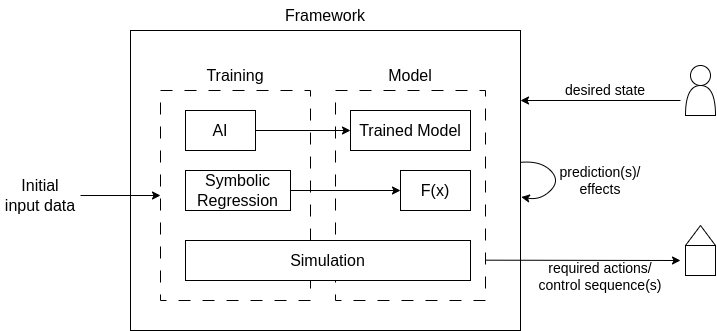
\includegraphics[width=.75\textwidth]{sample_architecture.png}
    \caption{Sample framework architecture}
\end{figure}

\newpage
As previously mentioned, the framework should be given some initial input data to train and/or model the smart home's environment and behavior.
Since there seems to be no best-practice yet for this explicit use-case, three different prediction techniques will be implemented:
\begin{itemize}
    \item[] \textbf{Artificial Intelligence model}.
        It needs to be considered what kind of artifical intelligence model fits this use-case the best, since there will be only sparse data to train with.
        The trained model will then be used to make predictions and figure out control sequences, given a desired state of the smart home.
        The aforementioned adaptability poses another challenge when dealing with artificial intelligence (more explicitly neural networks, etc.), as adding or removing smart devices also alters the input vector.
        Therefore an entire redesign and re-training of the model is required.
    \item[] \textbf{Symbolic Regression}.
        Approximating (property) functions is also a viable and interesting option, since it does not require a starting model but instead constructs the functions all on itself.
        The most interesting parts using symbolic regression (SR) are most likely going to be the accuracy of (different) SR algorithms working with a small data set and the overall applicability in this use-case.
    \item[] \textbf{Simulation model}.
        A simulation model would cover the Training- and Model-Phase, since a fully functioning simulation can be used for both.
        Additionally, the user initially not only needs to provide a set of real-world measurements but also the layout and arrangement of the smart home as well as some geo data.
        This would enable the simulation model to consider the real-world factors as day-night-cycle, weather as well as their effects on the smart home environment and its devices.
        Given the needed data, physical properties like brightness or temperature can be modeled/simulated.
\end{itemize}


\subsection{Validation \& Evaluation}
The main scientific contribution of this work will be the comparison between the three prediction techniques.
During the comparison, we will look at different factors like accuracy, amount of initial data needed (to function properly), efficiency and adaptability.
Before the evaluation, the findings will be validated using real-world measurements to confirm/falsify the prediction(s).

\newpage
\subsection{(Example) Structure}
\dirtree{%
    .1 .
    .2 Abstract (\textit{$\leftarrow$ actually needed?}).
    .2 1 Introduction.
    .2 2 Background.
    .2 3 Previous/Related Work.
    .2 4 Design.
    .3 4|1 What is the goal? How does it look (general architecture)?.
    .2 5 Implementation.
    .3 5|1 Available Data (small set of real world measurements).
    .3 5|2 Artificial Intelligence.
    .4 5|2|1 Network Model.
    .4 5|2|2 Training.
    .3 5|3 Simulation.
    .4 5|3|1 Base Model.
    .4 5|3|2 How to simulate temperature, brightness, etc..
    .4 5|3|3 What is used for simulation.
    .5 User input.
    .5 Inferred data.
    .3 5|4 Symbolic Regression.
    .4 5|4|1 Used method(s).
    .4 5|4|2 Results.
    .3 5|6 Validation (with real world data).
    .2 6 Evaluation.
    .3 6|1 Comparison between different implementations.
    .3 6|2 Discussion of (general) outcomes and findings.
    .2 7 Conclusion and Future Work.
}

%\section{Related Work}

\newpage
\section{Time Management}
% \subsection{Overview}
% \begin{table}[h!]
%     \begin{center}
%         \begin{tabular}{cccccc}
%             \toprule
%             \textbf{Week} & \textbf{Ch. 1 - 4} & \textbf{Implementation} & \textbf{Ch. 5 - 7} & \textbf{Buffer} \\
%             \midrule
%             1             & \checkmark         &                         &                    &                 \\
%             2             & \checkmark         &                         &                    &                 \\
%             3             & \checkmark         &                         &                    &                 \\
%             4             & \checkmark         &                         &                    &                 \\
%             5             &                    & \checkmark              &                    &                 \\
%             6             &                    & \checkmark              &                    &                 \\
%             7             &                    & \checkmark              &                    &                 \\
%             8             &                    & \checkmark              &                    &                 \\
%             9             &                    & \checkmark              &                    &                 \\
%             10            &                    & \checkmark              &                    &                 \\
%             11            &                    & \checkmark              &                    &                 \\
%             12            &                    & \checkmark              &                    &                 \\
%             13            &                    & \checkmark              &                    &                 \\
%             14            &                    & \checkmark              &                    &                 \\
%             15            &                    &                         & \checkmark         &                 \\
%             16            &                    &                         & \checkmark         &                 \\
%             17            &                    &                         & \checkmark         &                 \\
%             18            &                    &                         & \checkmark         &                 \\
%             19            &                    &                         & \checkmark         &                 \\
%             20            &                    &                         & \checkmark         &                 \\
%             21            &                    &                         & \checkmark         &                 \\
%             22            &                    &                         & \checkmark         &                 \\
%             23            &                    &                         &                    & \checkmark      \\
%             24            &                    &                         &                    & \checkmark      \\
%             25            &                    &                         &                    & \checkmark      \\
%             26            &                    &                         &                    & \checkmark      \\
%             \bottomrule
%         \end{tabular}
%     \end{center}
% \end{table}

%\subsection{Detailed Time List}
\begin{minipage}[t]{.45\textwidth}
    \textbf{Week 1-2}
    \begin{itemize}
        \item Ch. 1 Introduction
        \item Ch. 4 Design
        \item Collection of real-world data for training the framework later on
        \item Researching fitting prediction techniques (what AI models, what type of SR, simulation environment, etc.)
    \end{itemize}
    \textbf{Week 5-6}
    \begin{itemize}
        \item Implementing AI approach
        \item[]
        \item[]
    \end{itemize}
    \textbf{Week 9-10}
    \begin{itemize}
        \item Ch. 5.4 Symbolic Regression
        \item Implementing Simulation
    \end{itemize}
    \textbf{Week 13-14}
    \begin{itemize}
        \item Ch. 5.3 Simulation
        \item Ch. 5.4 Validation
        \item[]
        \item[]
    \end{itemize}
    \textbf{Week 17-18}
    \begin{itemize}
        \item Ch. 6 Evaluation
    \end{itemize}
    \textbf{Week 21-22}
    \begin{itemize}
        \item Ch. 2 Background
        \item Ch. 3 Previous/Related Work
    \end{itemize}
    \textbf{Week 25-26}
    \begin{itemize}
        \item Buffer
    \end{itemize}
\end{minipage}
\hfill
\begin{minipage}[t]{.45\textwidth}
    \textbf{Week 3-4}
    \begin{itemize}
        \item Researching fitting prediction techniques
        \item Ch. 5.1 Implementation/Available Data
        \item Implementation: Setting up framework
        \item[]
    \end{itemize}
    \textbf{Week 7-8}
    \begin{itemize}
        \item Ch. 5.2 Artifial Intelligence
        \item Implementing Symbolic Regression approach
    \end{itemize}
    \textbf{Week 11-12}
    \begin{itemize}
        \item Implementing Simulation
        \item[]
    \end{itemize}
    \textbf{Week 15-16}
    \begin{itemize}
        \item Connecting approaches inside the framework
        \item Rewriting code/Adaptions might be necessary
    \end{itemize}
    \textbf{Week 19-20}
    \begin{itemize}
        \item Ch. 7 Conclusion \& Future Work
    \end{itemize}
    \textbf{Week 23-24}
    \begin{itemize}
        \item Buffer
    \end{itemize}
\end{minipage}
\end{document}
